% !TEX root = ../main.tex
\subsection*{The Five Moons}

\begin{table*}[b]%
    \begin{DndTable}[width=\linewidth]{X}
        \centering
        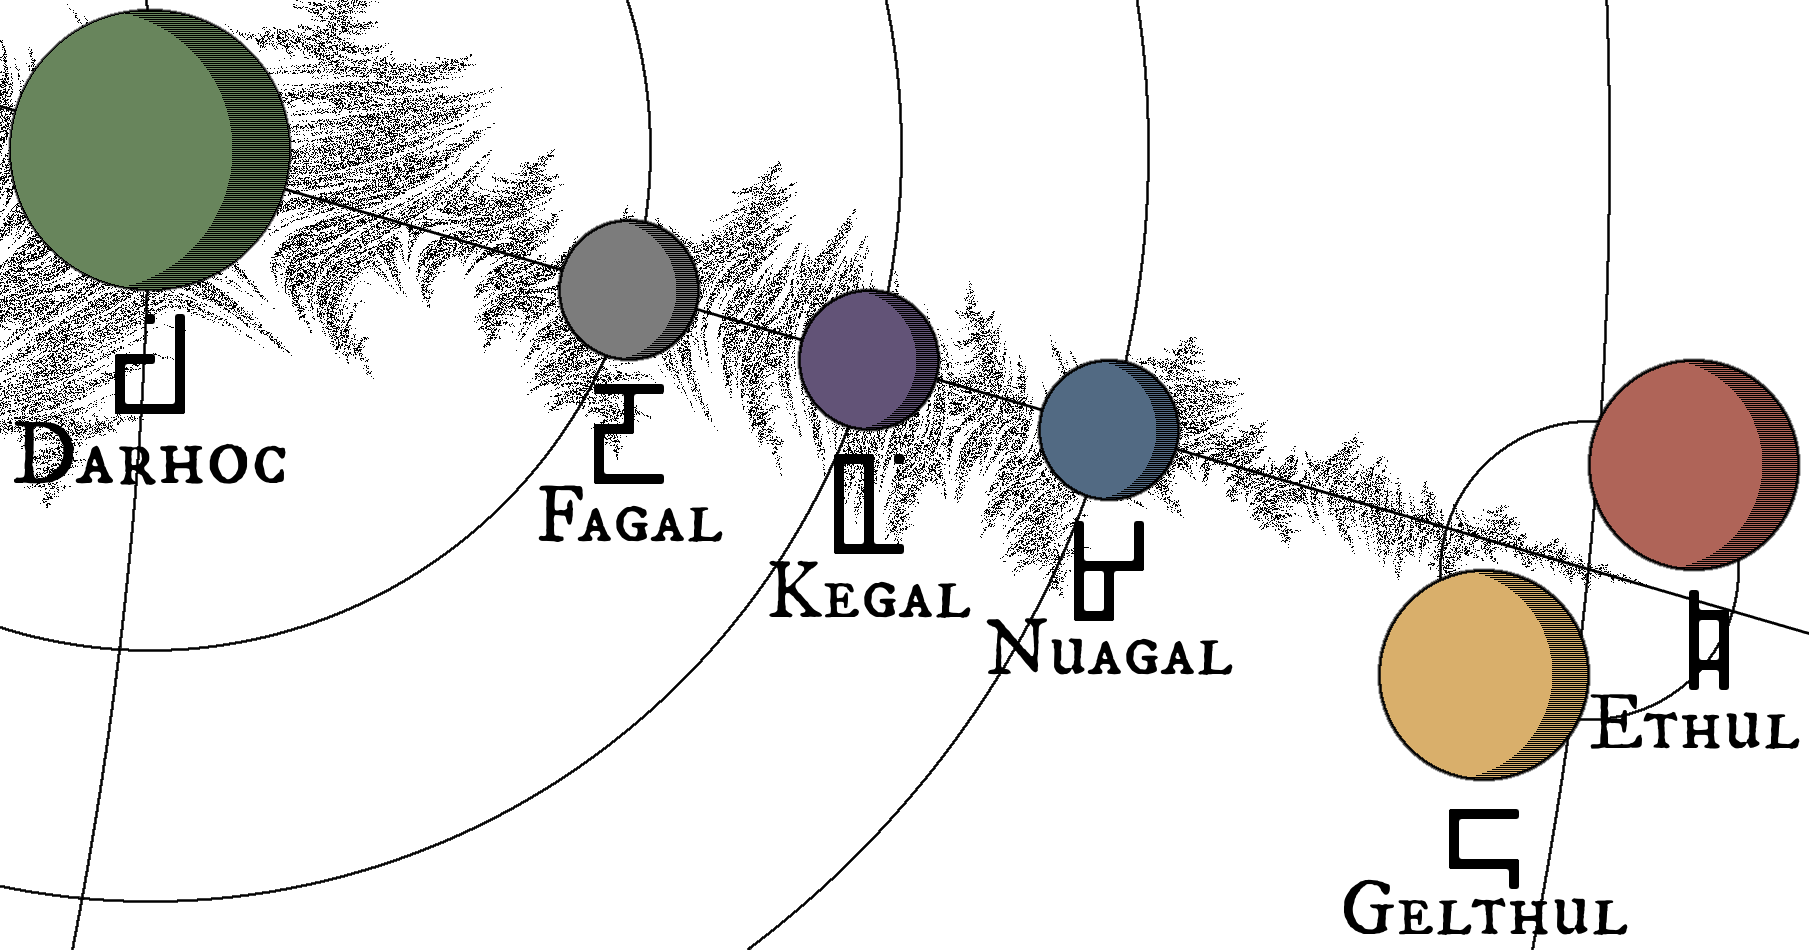
\includegraphics[width=0.99\textwidth]{01yuadrem/img/42moons.png}
    \end{DndTable}
\end{table*}

It is an undeniable fact of nature that moons have a strong effect over the tides.
In Yuadrem, this effect acts both on the ocean's tides and on the inviolate tides of the sentient mind.
Any religion or theory that attempts to explain the tides has to take the moons into consideration, for the two are intrinsecally linked.

The presence of three moons has interesting effects on the ocean tides.
Additionally, the ocassional influence of the twin planets of Rhelath adds more chaos to the system.
For centuries the tides were thought to be unpredictable, as impulsive and erratic as the whims of the mind.

This was until the then unknown oths of Abipolash designed the Nuagalian calendar.
Setting a year to two full translations of Nuagal, it predicts with astonishing accuracy the ocean's tides.
The ability to predict the tides enabled sailors to minimize risk in their journeys.
Some claim that only thanks to this calendar has the Whaler's Sea become the hub of commerce it is today.

There are some who claim to have visited the moons, supposedly through roads paved by the ets of yore.
While there is no substantial evidence to any of these claims, the vivid tales told by these explorers have left many to wonder.

While technically Yuadrem has three moons, the influence of the twin planets of Rhelath over the tides has made history count them as two additional moons.
A list of the moons along with a short description of each is provided.

\pagebreak

\subparagraph{Fagal} The largest and brightest object of the night sky, it is clear that Fagal seeks to be known by all people.
The patron moon of the Silver Tide, Fagal has the strongest influence over Yuadrem's tides, the water rising to kiss its gleaming face.
Its translation period is of 24 days, and its new moon marks the beginning of each month in the Fagalian calendar --- the most common calendar in Yuadrem.

\subparagraph{Kegal} Taking its place behind Fagal, Kegal takes its time to orbit Darhoc, observing even the loneliest commoner.
The patron moon of the Magenta Tide, Kegal's ever watchful eye is always attentive --- and judging --- of mortal lives.
Its translation period is of 48 days, and it is tidally locked to Yuadrem.

\subparagraph{Nuagal} The last of Darhoc's natural moons, Nuagal seems to mind its own business.
Intronspective and absorved, the patron moon of the Blue Tide holds no concern over mortal toil.
Its translation period is of 72 days, rotating freely and independant of Darhoc.

\subparagraph{Rhelath} The patron moons of the Gold and Red Tides respectively, Gelthul and Ethul are two planets locked in an eternal --- and deadly --- dance.
Some say that this dance represents the fiery fight inside oneself, the pull towards helping yourself against helping others.
% Roughly completing an orbit around each other twice a day, each moment that passes these two giants come closer to their eventual crash.

Gelthul and Ethul have orbitted each other for as long as sentience has existed in Yuadrem.%, and all predictions point to this continuing for the countless millenia to come.
The twin planets complete an orbit around Zash every 115 days, and approaches Darhoc every 169 days, wrecking havoc on the tides during their visit.

\pagebreak
